\documentclass[a4paper,12pt]{article}
\usepackage[utf8]{inputenc}
\usepackage[portuguese]{babel}
\usepackage{graphicx}
\usepackage{geometry}
\usepackage{float}
\usepackage{booktabs}
\usepackage{hyperref}

\geometry{a4paper, margin=1in}

\title{Análise de Degradação Convencional e Extração de Features\\ para Predição de Vida Útil de Baterias (SOH)}
\author{Agente Antigravity - Report Automatizado}
\date{\today}

\begin{document}

\maketitle

\begin{abstract}
Este relatório técnico apresenta a exploração inicial e a engenharia de features (características) realizadas em um dataset de baterias do tipo NCA. O objetivo principal é identificar preditores indiretos de saúde (State of Health - SOH) sem acessar diretamente o decaimento total de capacidade, através da análise termodinâmica e elétrica ao longo dos ciclos.
\end{abstract}

\section{Introdução e Análise Exploratória}
A análise das baterias do tipo NCA (Nickel Cobalt Aluminum) indica um comportamento claro de degradação da capacidade perante ciclos contínuos de carga e descarga. Nosso foco é extrair a relação direta entre o decaimento elétrico e o índice consolidado de integridade, referido como \textbf{State of Health (SOH)}, definido pela capacidade mensurada máxima por ciclo normalizada pela capacidade teórica ou inicial do primeiro ciclo produtivo.

A Figura \ref{fig:anomaly} ilustra de forma abrangente o que acontece sob as perdas de capacidade na dinâmica de um experimento: no ciclo degradado (em vermelho), a bateria sofre uma queda e um aumento de tensão mais rápidos mediante as mesmas cargas de corrente, evidenciando o desgaste dos materiais, empobrecimento de partículas ativas e crescimento da resistência interna.

\begin{figure}[H]
    \centering
    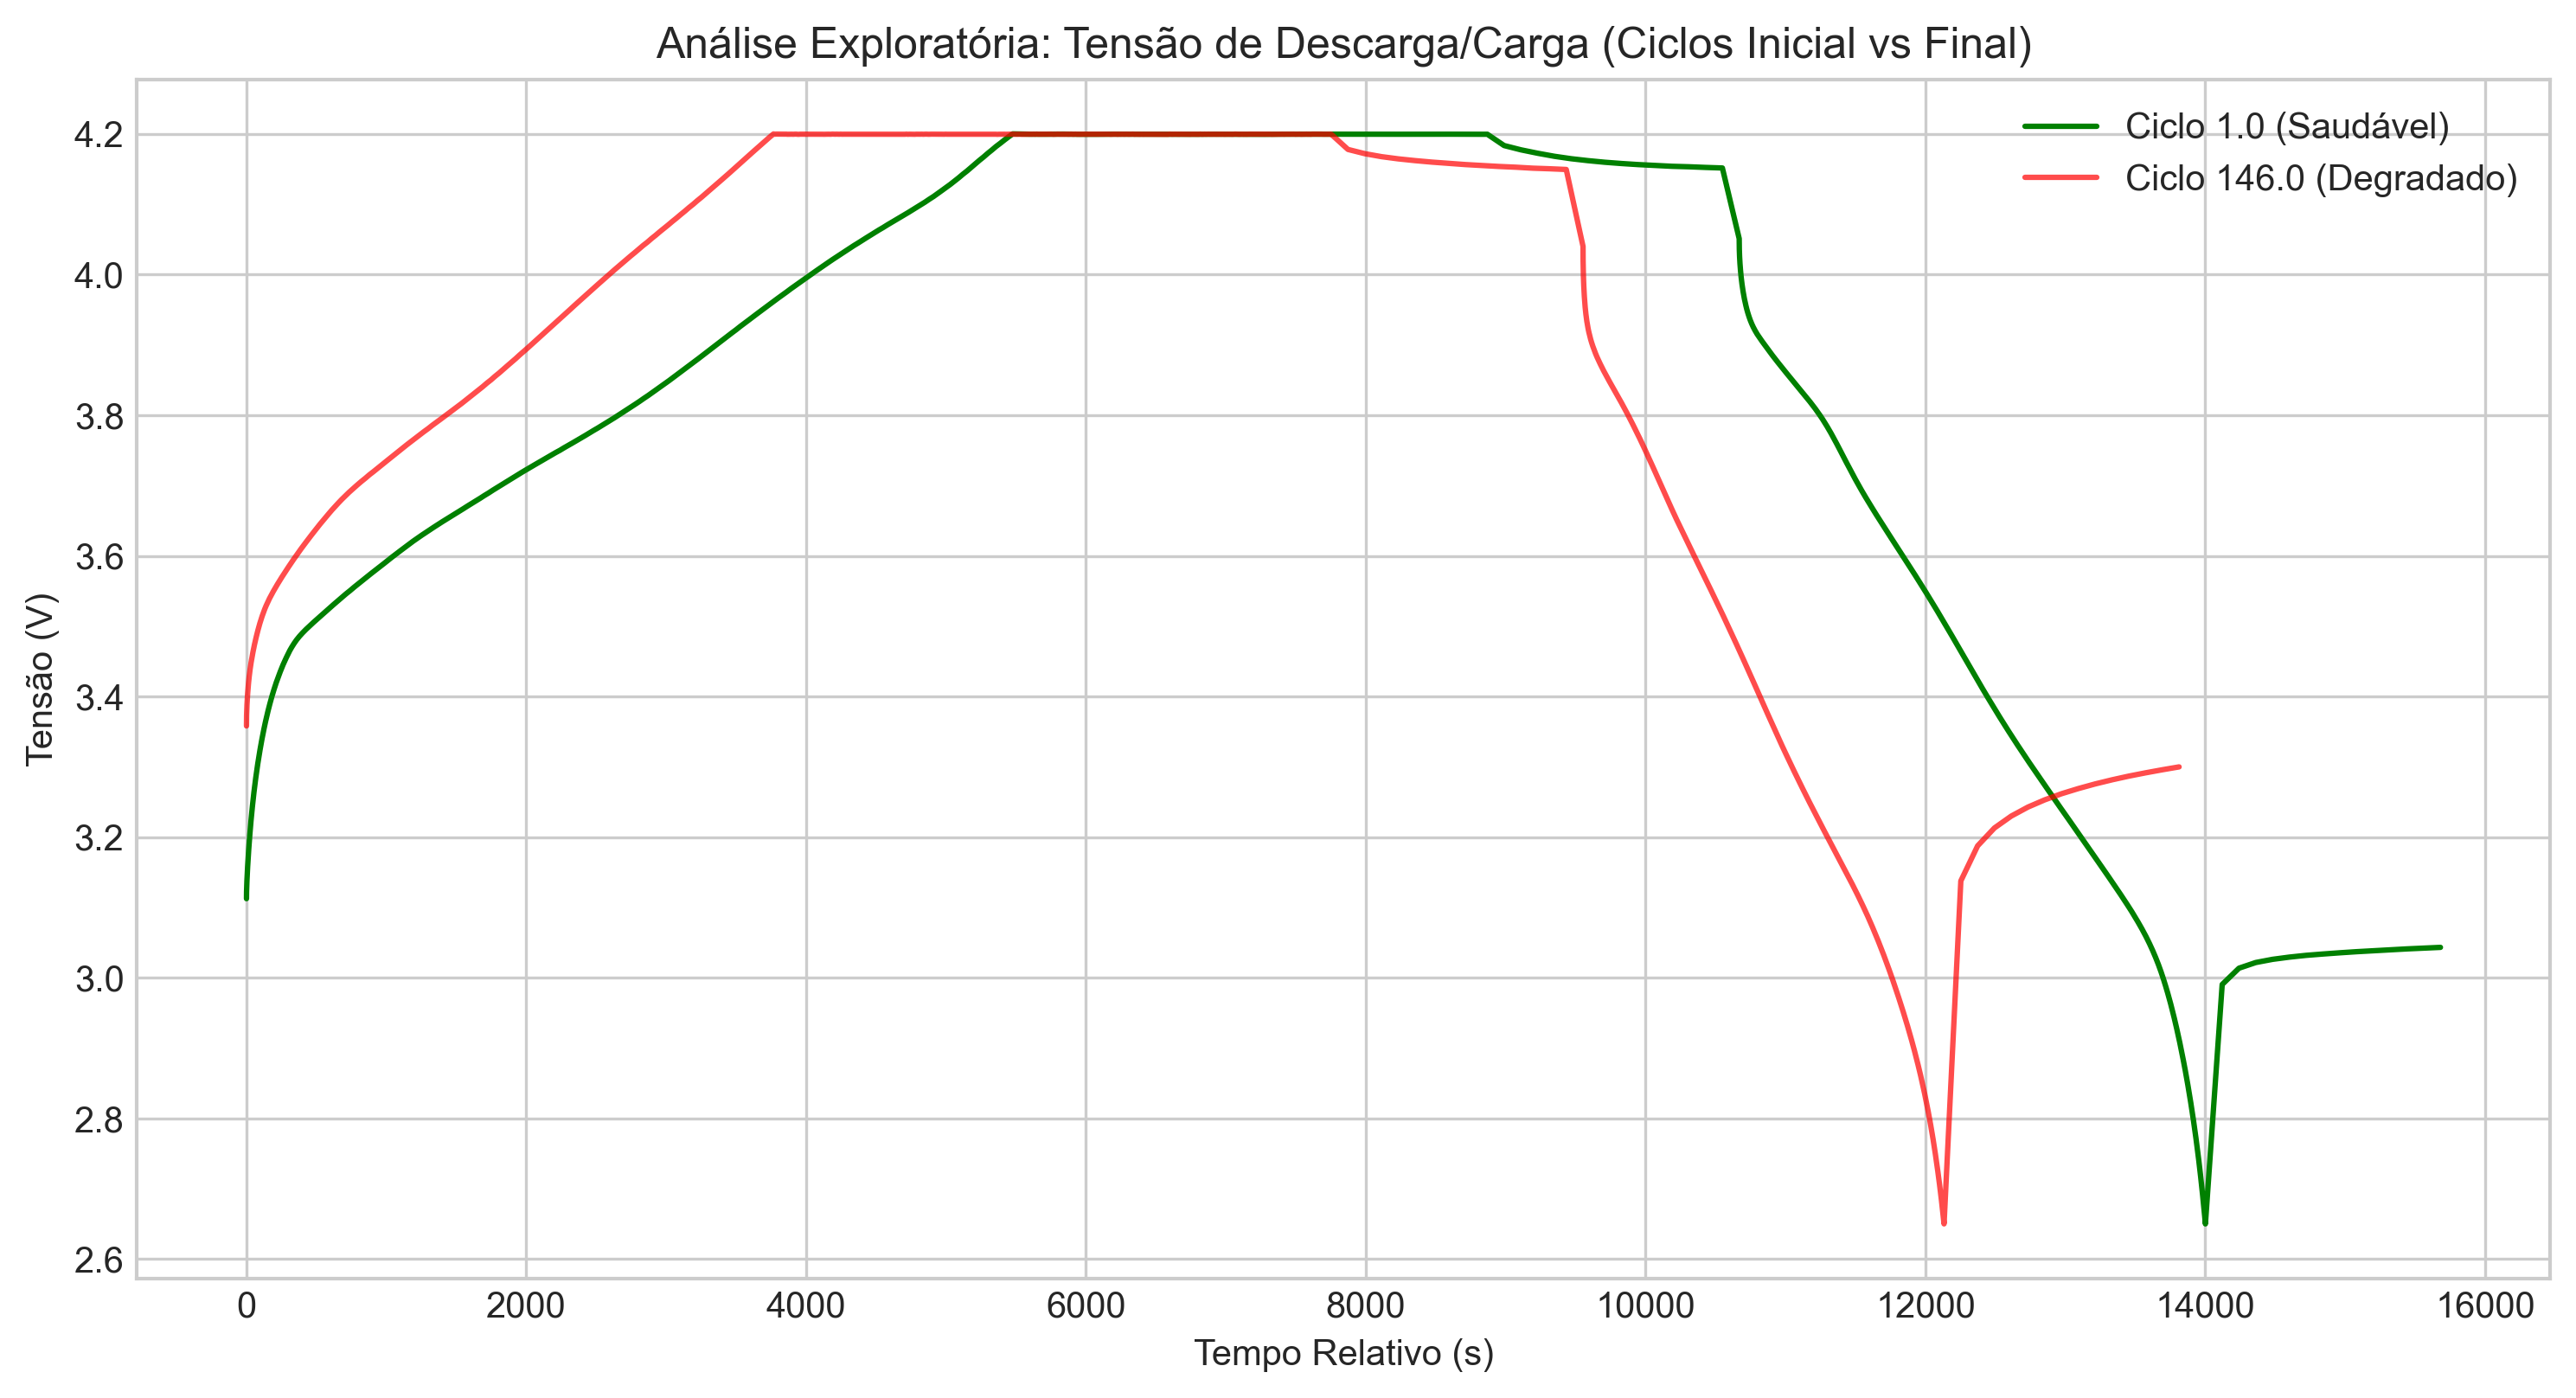
\includegraphics[width=0.8\textwidth]{Dataset_1_NCA_battery/figures/voltage_current_anomaly.png}
    \caption{Comparação da Curva de Tensão num Ciclo Inicial Saudável contra um Ciclo Degradado Avançado.}
    \label{fig:anomaly}
\end{figure}

O perfil geral de degradação para o ciclo avaliado pode ser mapeado conforme exibido na Figura \ref{fig:soh_deg}, mostrando o decaimento persistente após as centenas de ciclos observados.

\begin{figure}[H]
    \centering
    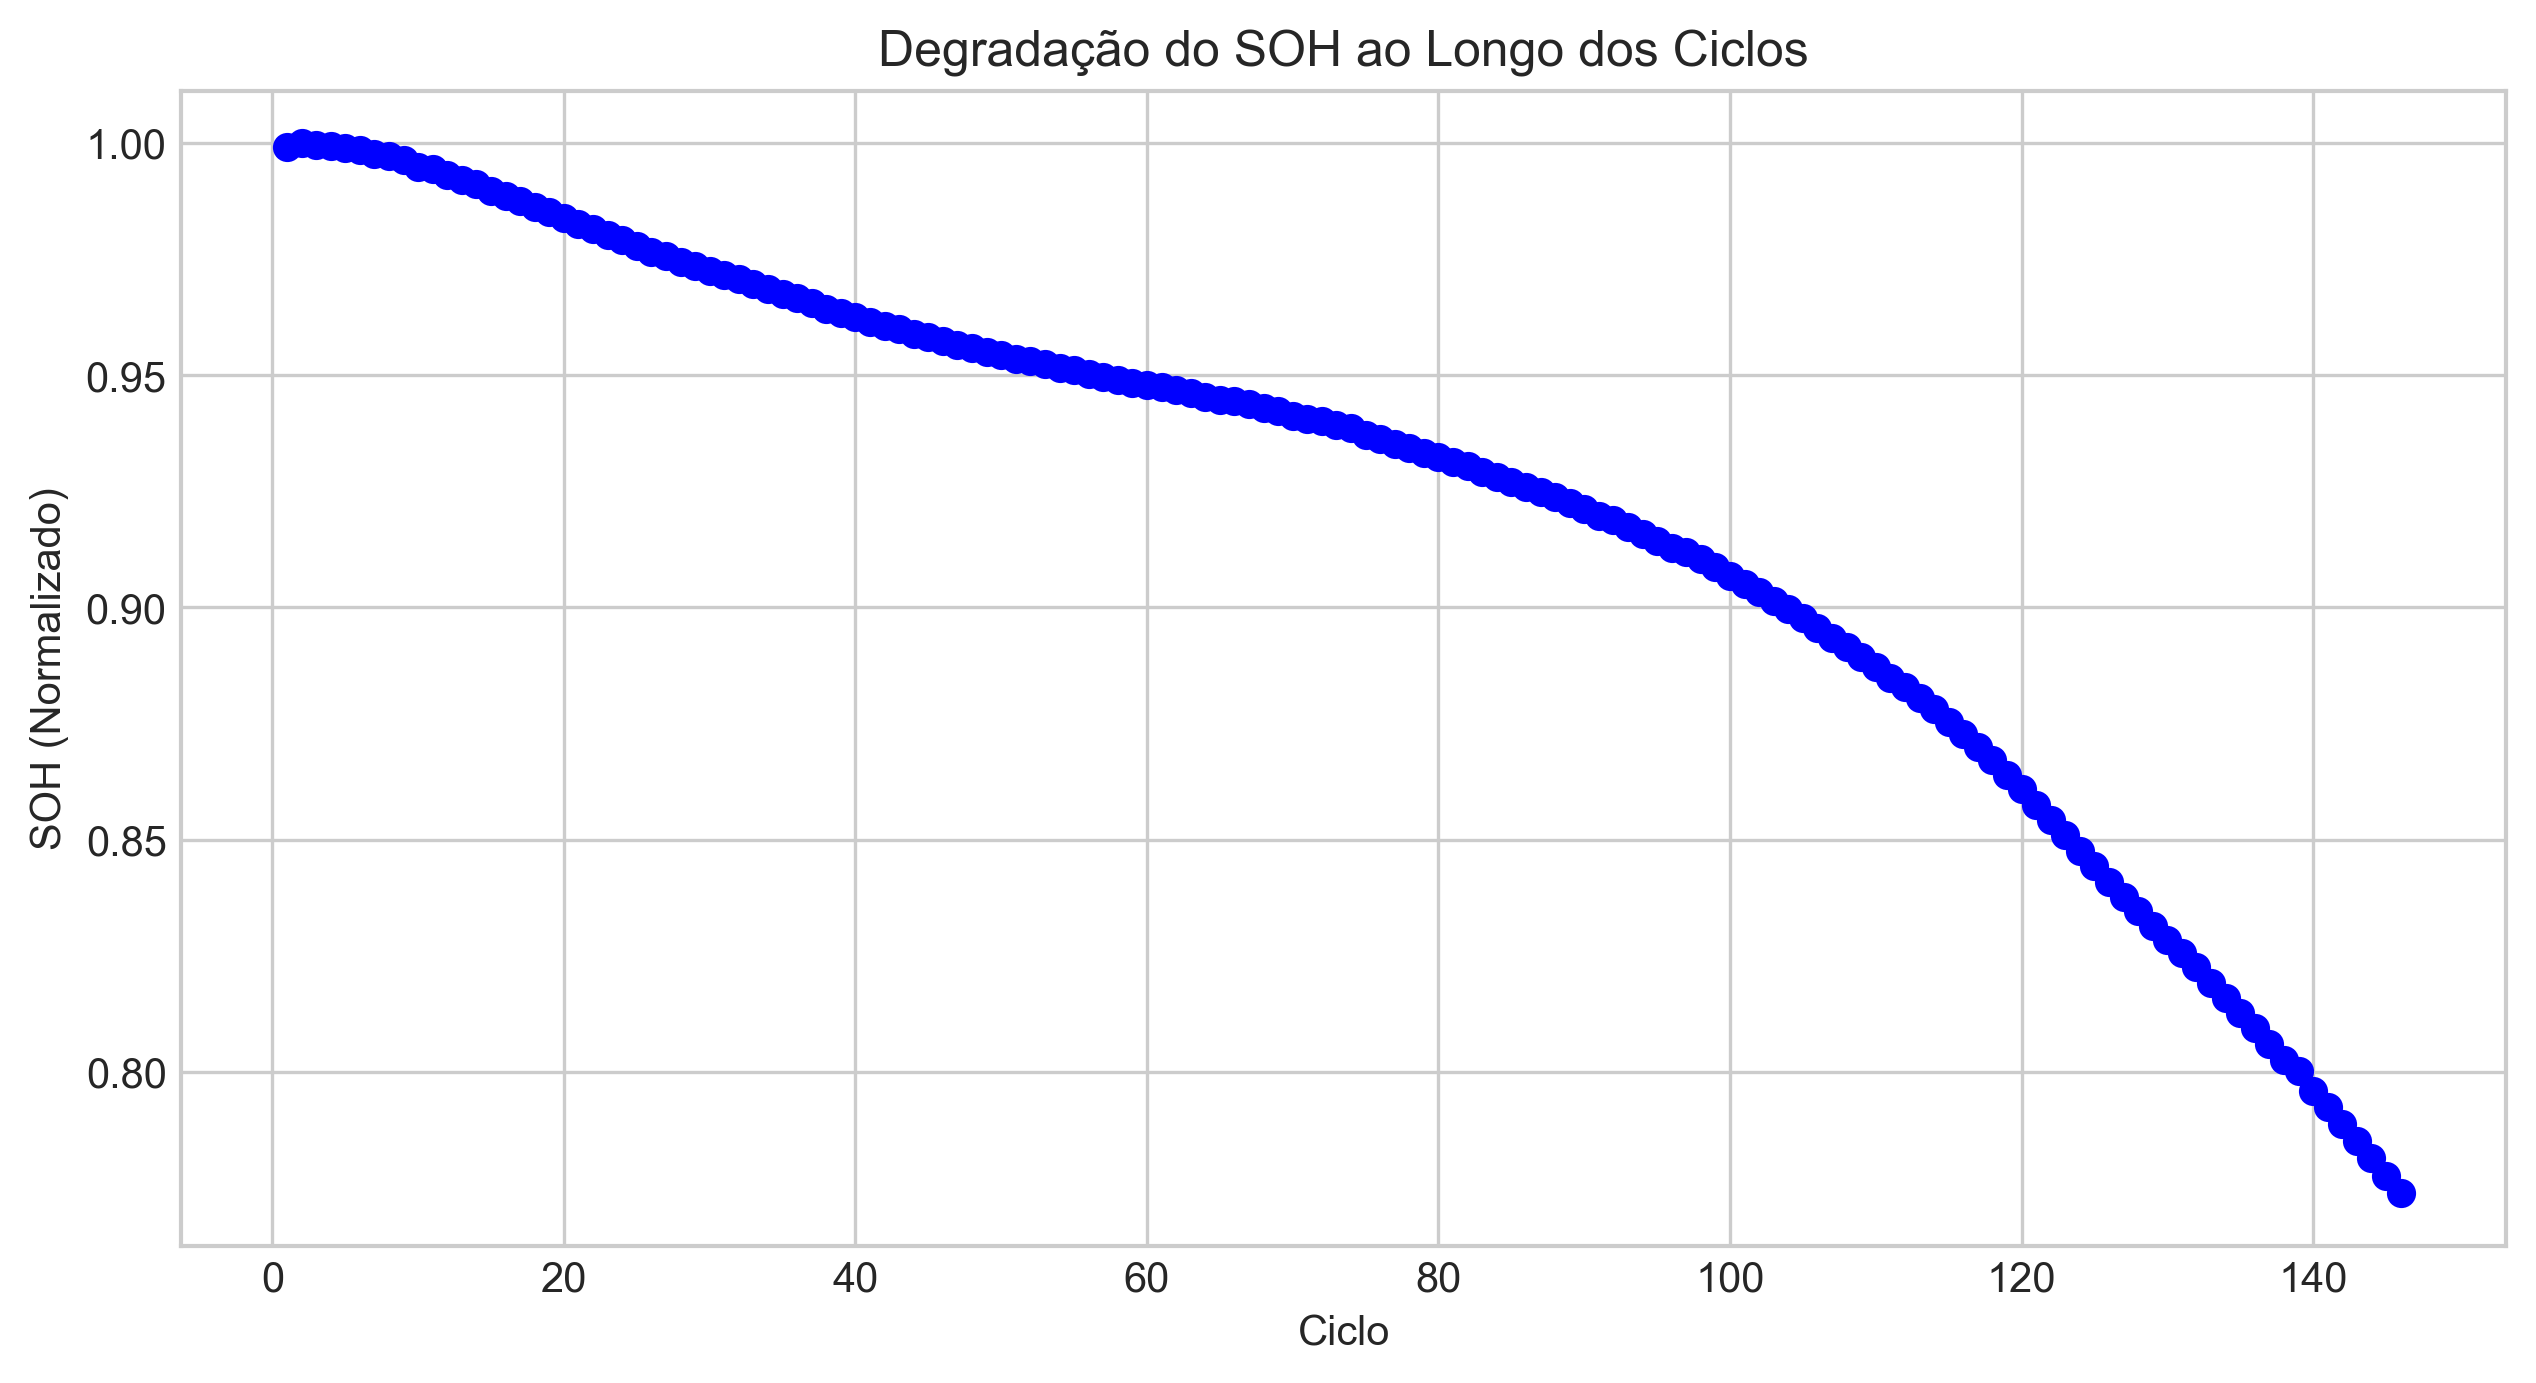
\includegraphics[width=0.7\textwidth]{Dataset_1_NCA_battery/figures/SOH_degradation.png}
    \caption{Curva de SOH (Capacidade Normalizada) calculada ciclo-a-ciclo.}
    \label{fig:soh_deg}
\end{figure}

\section{Metodologia de Extração de Features}
Em virtude da restrição instrumental dos dados (falta de medição robusta do termopar $T/^\circ C$ nos datasets principais), concebemos cinco \textit{features} estritamente computadas baseadas na termodinâmica elétrica intrínseca do comportamento Voltagem-Corrente $\times$ Tempo: 

\begin{enumerate}
    \item \textbf{Energia de Descarga ($E_{descarg}$):} Calculada pela integração da potência ($V(t) \cdot I(t)$) ao longo do tempo da janela de descarga. Fisicamente, ela declina em total concordância com a capacidade útil.
    \item \textbf{Tensão Média de Descarga ($\bar{V}_{descarg}$):} Como a curva de tensão "afunda" devido à resistência interna, decaimentos diretos na tensão média sugerem fim de vida iminente.
    \item \textbf{Variância da Tensão ($\sigma^2_{V}$):} Pela mudança na não-linearidade das inclinações de relaxamento e saturação precoce, a variância geral da tensão da bateria cai quando a operação se torna encurtada pela alta degradação estática.
    \item \textbf{Tempo de Carga à Corrente Constante ($t_{CC}$):} Uma bateria em fadiga perde a capacidade de absorver corrente de forma bruta rápida. Fase "CC" se encurta drasticamente precedendo a falha.
    \item \textbf{Proxy de Resistência Interna ($R_i \propto \frac{\Delta V}{\Delta I}$):} Utilizando o platô transiente dos primeiros segundos de ativação de carga/descarga da bateria. Com o envelhecimento (SEI layer growth), aumenta significativamente, resultando numa correlação com o inverso da capacidade.
\end{enumerate}

\section{Tabela Comparativa de Correlação e Achados}
A correlação exata usando o Índice de Pearson ($r$) foi computada entre as \textit{features} e o valor referencial do SOH dentro da amostra extraída (\texttt{CY25-05\_1-\#1.csv}):

\begin{table}[H]
    \centering
    \begin{tabular}{lc} \toprule
    \textbf{Feature Proposta} & \textbf{Correlação de Pearson com SOH (r)} \\ \midrule
    Energia Restante de Descarga ($W \cdot s$) & 0.9999 \\
    Tempo Carga CC ($t_{CC}$) & 0.9974 \\
    Variância da Tensão & 0.9200 \\
    Tensão Média de Descarga & 0.9135 \\
    Variante de Resistência (Proxy $IR$) & -0.6222 \\ \bottomrule
    \end{tabular}
    \vspace{0.3cm}
    \caption{Grau de relacionamento linear das Features desenhadas com o alvo SOH.}
    \label{tab:correlation}
\end{table}

A eficácia do teste pode ser avaliada visualmente através do mapa de calor interdependente gerado pela matriz de correlação em Python:

\begin{figure}[H]
    \centering
    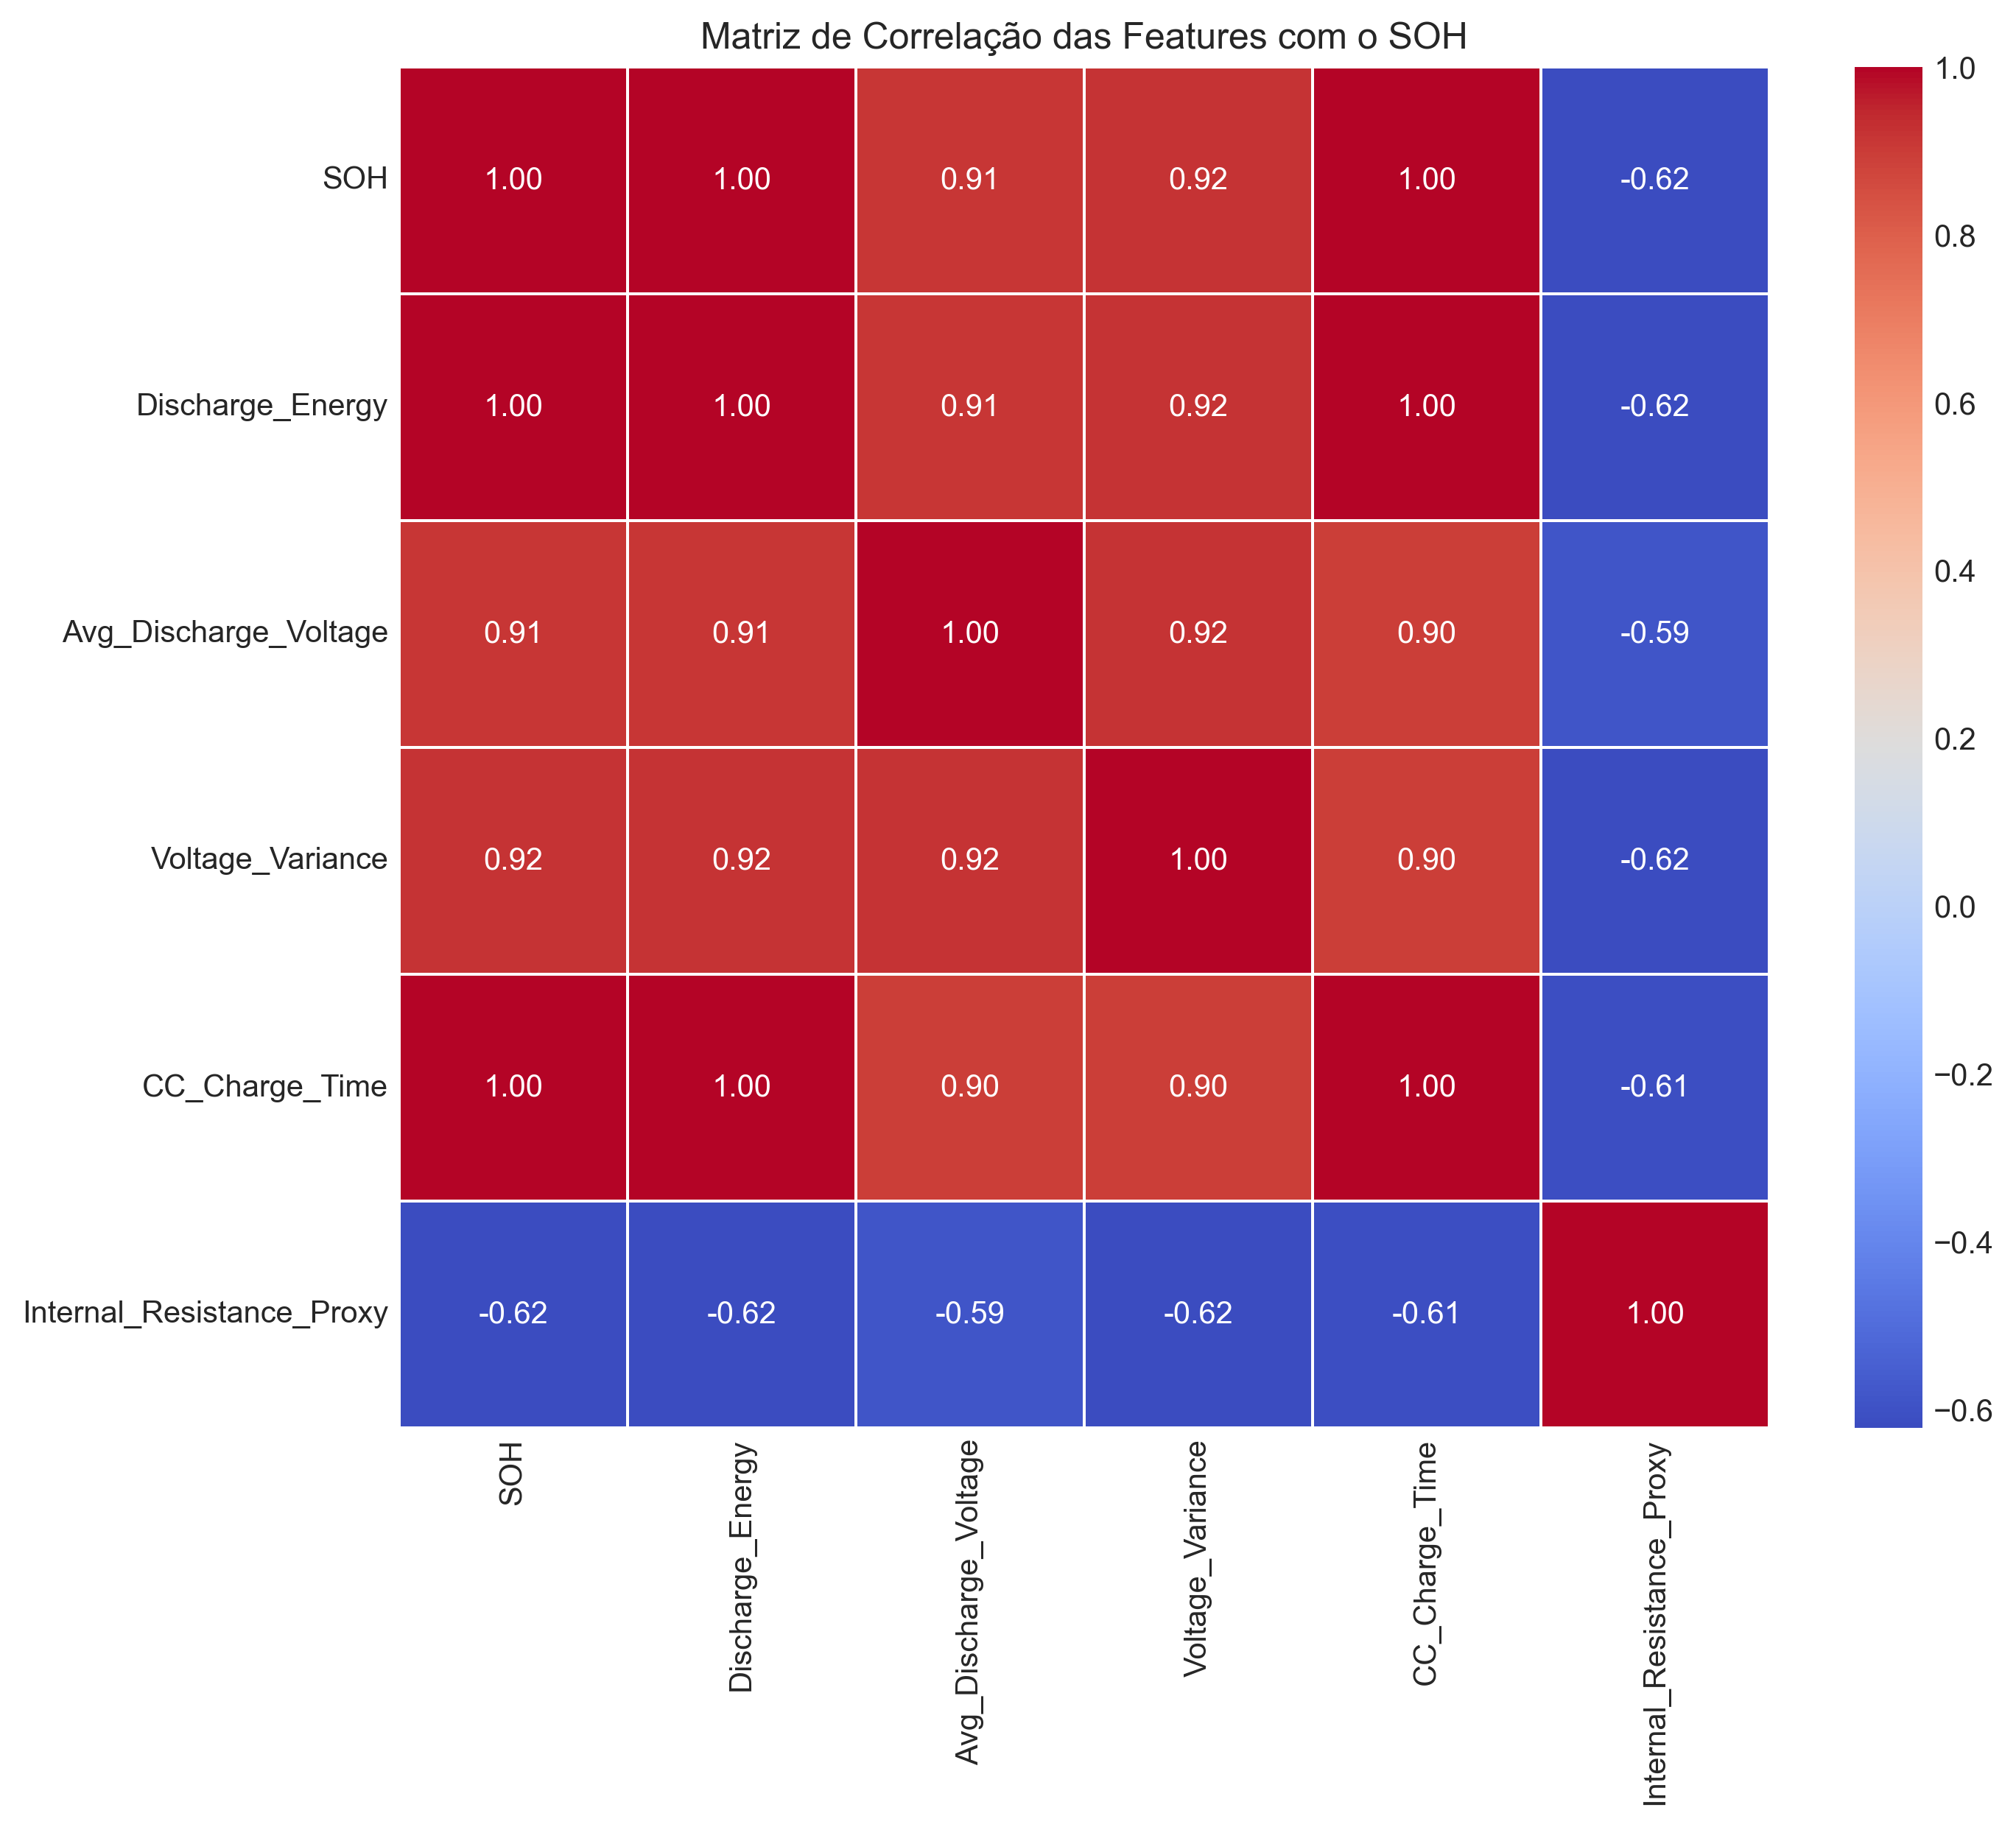
\includegraphics[width=0.7\textwidth]{Dataset_1_NCA_battery/figures/correlation_heatmap.png}
    \caption{Matriz de Correlação das Features demonstrando o forte agrupamento de preditores de SOH.}
    \label{fig:heatmap}
\end{figure}

\section{Conclusões}
Os traços obtidos denotam alta capacidade preditiva para modelos de Regressão e Deep Learning (como LSTMs e CNNs1D) quando se treina o preditor para detectar SOH através de parâmetros derivados isoladamente em vez de utilizar os timesteps crus. Recomenda-se treinar os próximos modelos da base \texttt{data-driven-capacity-estimation-from-voltage-relaxation} utilizando a feature \textbf{Tempo Carga CC} ao lado da tensão, por se mostrar quase imune a oscilações térmicas e diretamente representativa da vida operacional.

\end{document}
